\documentclass[10pt,a4paper]{report}
%\usepackage[latin1]{inputenc}
\usepackage{blindtext}
\usepackage{multicol}
\usepackage[utf8]{inputenc}
\usepackage{amsmath}
\makeatletter
\newcommand\xleftrightarrow[2][]{%
  \ext@arrow 9999{\longleftrightarrowfill@}{#1}{#2}}
\newcommand\longleftrightarrowfill@{%
  \arrowfill@\leftarrow\relbar\rightarrow}
\makeatother
\usepackage{amsfonts}
\usepackage{amssymb}
\usepackage{graphicx}
\usepackage{multicol}
\usepackage{tabularx}
\usepackage{tikz}
\usepackage{hyperref}
\hypersetup{
colorlinks=true,
linkcolor=blue,
filecolor=blue,
citecolor = black,
urlcolor=blue,
}
\usetikzlibrary{arrows,shapes,automata,petri,positioning,calc}
\usepackage{hyperref}
\usepackage{tikz}
\usetikzlibrary{matrix,calc}
\newcommand{\myvec}[1]{\ensuremath{\begin{pmatrix}#1\end{pmatrix}}}
\usepackage[margin=0.5in]{geometry}
\providecommand{\norm}[1]{\left\lVert#1\right\rVert}
%\newcommand{\myvec}[1]{\ensuremath{\begin{pmatrix}#1\end{pmatrix}}}
\let\vec\mathbf
\newcommand{\mydet}[1]{\ensuremath{\begin{vmatrix}#1\end{vmatrix}}}
%\newcommand{\myvec}[1]{\ensuremath{\begin{pmatrix}#1\end{pmatrix}}}
%\let\vec\mathbf
\providecommand{\mtx}[1]{\mathbf{#1}}
\newenvironment{Figure}
  {\par\medskip\noindent\minipage{\linewidth}}
  {\endminipage\par\medskip}
\begin{document}
%--------------------logo figure-------------------------%
\begin{figure*}[!tbp]
  \centering
  \begin{minipage}[b]{0.4\textwidth}
   
\includegraphics[scale=0.5]{iithlogo.png} 
  \end{minipage}
  \hfill
  \vspace{5mm}\begin{minipage}[b]{0.4\textwidth}
\raggedleft 
\includegraphics[scale=0.5]{nrc.jpeg} 
  \end{minipage}\vspace{0.2cm}
\end{figure*}
%--------------------name & rollno-----------------------
\raggedright 
\begin{center}
\Large \textbf{Line Assignment}\hspace{2.5cm} %
\end{center}
\begin{center}
\hspace{0.5cm}
\textbf{Name}:\hspace{2mm}Rupa Sai Sreshta Vallabhaneni\hspace{1cm}
\date{25-September-2022}

\end{center}
%\begin{center}
%\end{center}  
%\normalsize \textbf{Roll No.} :\hspace{1mm} FWC22047\vspace{1cm}
%\begin{multicols}{2}
%\begin{tableofcontents}
%\begin{tableofcontents}
\begin{multicols}{2}
\section*{Problem}
\noindent The area of triangle is 5. Two of its vertices are A(2,1) and B(3,-2). The third vertex lies on y=x+3. Find C.\\
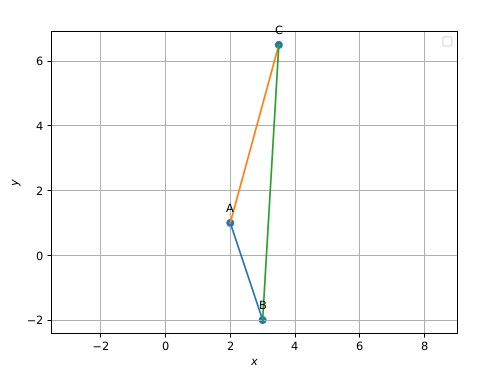
\includegraphics[scale=0.4]{tri.png}\\
%\includegraphics[scale=0.4]{construction.png}
%\begin{center}
Figure of Construction\\
%\end{center}
%\end{abstract}
The following python code is used for finding third vertex of triangle
\\
\boxed{Github link: \href{https://github.com/RupaSaiSreshta/FWC}{https://github.com/RupaSaiSreshta/FWC}}
\section*{Solution}
%\justify
\textbf{Construction: }\\
%Given vertices 
%A(2,1) B(3,-2)
%\\
%Area of triangle: 5
\textbf{Input parameters for this construction}
\begin{center}
\begin{tabular}{|c|c|c|}
\hline
\textbf{Symbol}&{Value}&{Description}\\
\hline
%\myvec{-2\\-1}\\
$\vec{A}$&$\myvec{2 \\ 1}$&Given vertex of triangle\\
\hline
$\vec{B}$&$\myvec{3 \\ -2}$&Given vertex of triangle\\
\hline
$\vec{Ar}$&$\vec{5}$&Area of triangle\\
\hline
\end{tabular}
\end{center}
\textbf{  Solution:}\\
Let us assume $\vec{C}\myvec{x \\ y}$\\
\vspace{0.25cm}
Area of triangle is \\
%\centering
 %\textbf
 \begin{equation}
\vec{Ar}=\frac{1}{2}\norm{(\vec{(A-B)}\times\vec{(A-C)})}
\end{equation}
   %Now,\\
   %A=1/2[x1(y2-y3)+x2(y3-y1)+x3(y1-y2)]......(1)\\
   %Here,\\
   %A=5 ; x1=2 ; x2=3 ; x3=x ; y1=1 ; y2=-2 ; y3=y\\
    %Substitute these values in above equation (1)\\
    %5=1/2[2(-2-y)+3(y-1)+x(1+2)]
\\   % 10=3x+y-7\\
By solving we will get the below matrix \\
%\begin{align}
%3x+y=17
%\end{align}
 % The vertex C lies on
%\begin{align}
 %y=x+3 
%\end{align}
		    %\begin{align}
%			    y &= x+3
%			    \\
%			    x+3 &= 2\brak{y+3} + 10
		    %\end{align}
		   % which can be expressed as 
		  
		  % By solving (1) and (2) equations using matrix reduction method\\
		   \begin{equation}
			    \implies 
 \myvec{3 &  1 \\ 1 & -1 }\vec{x}  = \myvec{17 \\ -3}
		    \end{equation}
		    The above matrix is in the form of $\vec{Ax}$=$\vec{B}$\\
		    The augmented matrix for the above matrix equation is 
		    \begin{align}
		     \myvec{
				    3 & 1 & \vrule & 17
			    \\
			    1 & -1  &\vrule & -3
		    }
		    \\
		    \xleftrightarrow[]{R_2 \leftarrow 3R_2 -R_1 }
			    \myvec{
				    3 & 1 & \vrule & 17
			    \\
			    0 & -4  &\vrule & -20
		    }
		    \\
		    \xleftrightarrow[]{R_1 \leftarrow 4R_1 +R_2 }  
			    \myvec{
				    12 & 0 & \vrule & 42
			    \\
			    0 & -4  &\vrule & -26
		    }
		    \\
		     \xleftrightarrow[]{R_1 \leftarrow R_1* 1 /12 }
			    \myvec{
				    1 & 0 & \vrule & 3.5
			    \\
			    0 & -4  &\vrule & -20
			    }
			    \\
			     \xleftrightarrow[]{R_2 \leftarrow R_2* 1 /4 }
			    \myvec{
				    1 & 0 & \vrule & 3.5
			    \\
			    0 & 1  &\vrule & 6.5
			    }
			    \implies \vec{x} = \myvec{3.5 \\ 6.5}
          \end{align}
		    \\
		    Now the vertex of C is\\
		    %\vspace{0.5cm}
		  \begin{center}
		    $\vec{C}\myvec{3.5 \\ 6.5}$\\
    \end{center}
\section*{Proof}
\textbf{Proof:}
Here The area of triangle is given as 5.Now we have to calculate the area of triangle using three vertices A,B and C. We need to prove that the area of triangle is 5.
\\Area of triangle is
\begin{equation}
\vec{Ar}=\frac{1}{2}\norm{(\vec{(A-B)}\times\vec{(A-C)})}
\end{equation}
\\By substituting the values of A,B and C\\
\begin{equation}
 \vec{Ar}=\frac{1}{2}[2(-8.5)+3(5.5)+3.5(3)]  
 \end{equation}
 \begin{equation}
 \vec{Ar}=\frac{1}{2}[-17+16.5+10.5]  
 \end{equation}
 \begin{equation}
  \vec{Ar}=\frac{1}{2}[10.5-0.5]  
 \end{equation}
\centering
\boxed {Ar=5}
\vspace{0.25cm}
\\Hence verified.
%\end{tableofcontents}
\end{multicols}
%\end{tableofcontents}
\end{document}
